% Options for packages loaded elsewhere
% Options for packages loaded elsewhere
\PassOptionsToPackage{unicode}{hyperref}
\PassOptionsToPackage{hyphens}{url}
\PassOptionsToPackage{dvipsnames,svgnames,x11names}{xcolor}
%
\documentclass[
  letterpaper,
  DIV=11,
  numbers=noendperiod]{scrartcl}
\usepackage{xcolor}
\usepackage{amsmath,amssymb}
\setcounter{secnumdepth}{-\maxdimen} % remove section numbering
\usepackage{iftex}
\ifPDFTeX
  \usepackage[T1]{fontenc}
  \usepackage[utf8]{inputenc}
  \usepackage{textcomp} % provide euro and other symbols
\else % if luatex or xetex
  \usepackage{unicode-math} % this also loads fontspec
  \defaultfontfeatures{Scale=MatchLowercase}
  \defaultfontfeatures[\rmfamily]{Ligatures=TeX,Scale=1}
\fi
\usepackage{lmodern}
\ifPDFTeX\else
  % xetex/luatex font selection
\fi
% Use upquote if available, for straight quotes in verbatim environments
\IfFileExists{upquote.sty}{\usepackage{upquote}}{}
\IfFileExists{microtype.sty}{% use microtype if available
  \usepackage[]{microtype}
  \UseMicrotypeSet[protrusion]{basicmath} % disable protrusion for tt fonts
}{}
\makeatletter
\@ifundefined{KOMAClassName}{% if non-KOMA class
  \IfFileExists{parskip.sty}{%
    \usepackage{parskip}
  }{% else
    \setlength{\parindent}{0pt}
    \setlength{\parskip}{6pt plus 2pt minus 1pt}}
}{% if KOMA class
  \KOMAoptions{parskip=half}}
\makeatother
% Make \paragraph and \subparagraph free-standing
\makeatletter
\ifx\paragraph\undefined\else
  \let\oldparagraph\paragraph
  \renewcommand{\paragraph}{
    \@ifstar
      \xxxParagraphStar
      \xxxParagraphNoStar
  }
  \newcommand{\xxxParagraphStar}[1]{\oldparagraph*{#1}\mbox{}}
  \newcommand{\xxxParagraphNoStar}[1]{\oldparagraph{#1}\mbox{}}
\fi
\ifx\subparagraph\undefined\else
  \let\oldsubparagraph\subparagraph
  \renewcommand{\subparagraph}{
    \@ifstar
      \xxxSubParagraphStar
      \xxxSubParagraphNoStar
  }
  \newcommand{\xxxSubParagraphStar}[1]{\oldsubparagraph*{#1}\mbox{}}
  \newcommand{\xxxSubParagraphNoStar}[1]{\oldsubparagraph{#1}\mbox{}}
\fi
\makeatother

\usepackage{color}
\usepackage{fancyvrb}
\newcommand{\VerbBar}{|}
\newcommand{\VERB}{\Verb[commandchars=\\\{\}]}
\DefineVerbatimEnvironment{Highlighting}{Verbatim}{commandchars=\\\{\}}
% Add ',fontsize=\small' for more characters per line
\usepackage{framed}
\definecolor{shadecolor}{RGB}{241,243,245}
\newenvironment{Shaded}{\begin{snugshade}}{\end{snugshade}}
\newcommand{\AlertTok}[1]{\textcolor[rgb]{0.68,0.00,0.00}{#1}}
\newcommand{\AnnotationTok}[1]{\textcolor[rgb]{0.37,0.37,0.37}{#1}}
\newcommand{\AttributeTok}[1]{\textcolor[rgb]{0.40,0.45,0.13}{#1}}
\newcommand{\BaseNTok}[1]{\textcolor[rgb]{0.68,0.00,0.00}{#1}}
\newcommand{\BuiltInTok}[1]{\textcolor[rgb]{0.00,0.23,0.31}{#1}}
\newcommand{\CharTok}[1]{\textcolor[rgb]{0.13,0.47,0.30}{#1}}
\newcommand{\CommentTok}[1]{\textcolor[rgb]{0.37,0.37,0.37}{#1}}
\newcommand{\CommentVarTok}[1]{\textcolor[rgb]{0.37,0.37,0.37}{\textit{#1}}}
\newcommand{\ConstantTok}[1]{\textcolor[rgb]{0.56,0.35,0.01}{#1}}
\newcommand{\ControlFlowTok}[1]{\textcolor[rgb]{0.00,0.23,0.31}{\textbf{#1}}}
\newcommand{\DataTypeTok}[1]{\textcolor[rgb]{0.68,0.00,0.00}{#1}}
\newcommand{\DecValTok}[1]{\textcolor[rgb]{0.68,0.00,0.00}{#1}}
\newcommand{\DocumentationTok}[1]{\textcolor[rgb]{0.37,0.37,0.37}{\textit{#1}}}
\newcommand{\ErrorTok}[1]{\textcolor[rgb]{0.68,0.00,0.00}{#1}}
\newcommand{\ExtensionTok}[1]{\textcolor[rgb]{0.00,0.23,0.31}{#1}}
\newcommand{\FloatTok}[1]{\textcolor[rgb]{0.68,0.00,0.00}{#1}}
\newcommand{\FunctionTok}[1]{\textcolor[rgb]{0.28,0.35,0.67}{#1}}
\newcommand{\ImportTok}[1]{\textcolor[rgb]{0.00,0.46,0.62}{#1}}
\newcommand{\InformationTok}[1]{\textcolor[rgb]{0.37,0.37,0.37}{#1}}
\newcommand{\KeywordTok}[1]{\textcolor[rgb]{0.00,0.23,0.31}{\textbf{#1}}}
\newcommand{\NormalTok}[1]{\textcolor[rgb]{0.00,0.23,0.31}{#1}}
\newcommand{\OperatorTok}[1]{\textcolor[rgb]{0.37,0.37,0.37}{#1}}
\newcommand{\OtherTok}[1]{\textcolor[rgb]{0.00,0.23,0.31}{#1}}
\newcommand{\PreprocessorTok}[1]{\textcolor[rgb]{0.68,0.00,0.00}{#1}}
\newcommand{\RegionMarkerTok}[1]{\textcolor[rgb]{0.00,0.23,0.31}{#1}}
\newcommand{\SpecialCharTok}[1]{\textcolor[rgb]{0.37,0.37,0.37}{#1}}
\newcommand{\SpecialStringTok}[1]{\textcolor[rgb]{0.13,0.47,0.30}{#1}}
\newcommand{\StringTok}[1]{\textcolor[rgb]{0.13,0.47,0.30}{#1}}
\newcommand{\VariableTok}[1]{\textcolor[rgb]{0.07,0.07,0.07}{#1}}
\newcommand{\VerbatimStringTok}[1]{\textcolor[rgb]{0.13,0.47,0.30}{#1}}
\newcommand{\WarningTok}[1]{\textcolor[rgb]{0.37,0.37,0.37}{\textit{#1}}}

\usepackage{longtable,booktabs,array}
\usepackage{calc} % for calculating minipage widths
% Correct order of tables after \paragraph or \subparagraph
\usepackage{etoolbox}
\makeatletter
\patchcmd\longtable{\par}{\if@noskipsec\mbox{}\fi\par}{}{}
\makeatother
% Allow footnotes in longtable head/foot
\IfFileExists{footnotehyper.sty}{\usepackage{footnotehyper}}{\usepackage{footnote}}
\makesavenoteenv{longtable}
\usepackage{graphicx}
\makeatletter
\newsavebox\pandoc@box
\newcommand*\pandocbounded[1]{% scales image to fit in text height/width
  \sbox\pandoc@box{#1}%
  \Gscale@div\@tempa{\textheight}{\dimexpr\ht\pandoc@box+\dp\pandoc@box\relax}%
  \Gscale@div\@tempb{\linewidth}{\wd\pandoc@box}%
  \ifdim\@tempb\p@<\@tempa\p@\let\@tempa\@tempb\fi% select the smaller of both
  \ifdim\@tempa\p@<\p@\scalebox{\@tempa}{\usebox\pandoc@box}%
  \else\usebox{\pandoc@box}%
  \fi%
}
% Set default figure placement to htbp
\def\fps@figure{htbp}
\makeatother





\setlength{\emergencystretch}{3em} % prevent overfull lines

\providecommand{\tightlist}{%
  \setlength{\itemsep}{0pt}\setlength{\parskip}{0pt}}



 


\KOMAoption{captions}{tableheading}
\makeatletter
\@ifpackageloaded{caption}{}{\usepackage{caption}}
\AtBeginDocument{%
\ifdefined\contentsname
  \renewcommand*\contentsname{Table of contents}
\else
  \newcommand\contentsname{Table of contents}
\fi
\ifdefined\listfigurename
  \renewcommand*\listfigurename{List of Figures}
\else
  \newcommand\listfigurename{List of Figures}
\fi
\ifdefined\listtablename
  \renewcommand*\listtablename{List of Tables}
\else
  \newcommand\listtablename{List of Tables}
\fi
\ifdefined\figurename
  \renewcommand*\figurename{Figure}
\else
  \newcommand\figurename{Figure}
\fi
\ifdefined\tablename
  \renewcommand*\tablename{Table}
\else
  \newcommand\tablename{Table}
\fi
}
\@ifpackageloaded{float}{}{\usepackage{float}}
\floatstyle{ruled}
\@ifundefined{c@chapter}{\newfloat{codelisting}{h}{lop}}{\newfloat{codelisting}{h}{lop}[chapter]}
\floatname{codelisting}{Listing}
\newcommand*\listoflistings{\listof{codelisting}{List of Listings}}
\makeatother
\makeatletter
\makeatother
\makeatletter
\@ifpackageloaded{caption}{}{\usepackage{caption}}
\@ifpackageloaded{subcaption}{}{\usepackage{subcaption}}
\makeatother
\usepackage{bookmark}
\IfFileExists{xurl.sty}{\usepackage{xurl}}{} % add URL line breaks if available
\urlstyle{same}
\hypersetup{
  pdftitle={Homework 3},
  pdfauthor={Owen Wright},
  colorlinks=true,
  linkcolor={blue},
  filecolor={Maroon},
  citecolor={Blue},
  urlcolor={Blue},
  pdfcreator={LaTeX via pandoc}}


\title{Homework 3}
\author{Owen Wright}
\date{2026-05-28}
\begin{document}
\maketitle

\renewcommand*\contentsname{Table of contents}
{
\hypersetup{linkcolor=}
\setcounter{tocdepth}{3}
\tableofcontents
}

\begin{Shaded}
\begin{Highlighting}[]
\CommentTok{\#Load the tidyverse package}
\FunctionTok{library}\NormalTok{(tidyverse)}

\CommentTok{\# Load the here package so file paths follow correctly}
\FunctionTok{library}\NormalTok{(here)}

\CommentTok{\#Read in the kelp data and store as an object called kelp}
\NormalTok{kelp }\OtherTok{\textless{}{-}} \FunctionTok{read\_csv}\NormalTok{(}\FunctionTok{here}\NormalTok{(}\StringTok{"data"}\NormalTok{, }\StringTok{"temp{-}kelp.csv"}\NormalTok{))}

\CommentTok{\#Read in personal data and store as an object called personal\_data}
\NormalTok{personal\_data }\OtherTok{\textless{}{-}} \FunctionTok{read\_csv}\NormalTok{(}\FunctionTok{here}\NormalTok{(}\StringTok{"data"}\NormalTok{, }\StringTok{"personaldata2.csv"}\NormalTok{))}
\end{Highlighting}
\end{Shaded}

\section{Problem 1. Giant kelp
fronds}\label{problem-1.-giant-kelp-fronds}

\subsection{a. An appropriate test}\label{a.-an-appropriate-test}

In order to determine the strength of the relationship between
temperature and giant kelp frond elongation rate, one may employ a
Pearson correlation test, which measures how strong the relationship is
and whether it is positive or negative. Additionally, one may utilize a
simple linear regression test to determine whether ocean temperature
predicts kelp elongation rate and what the growth rate is for each 1°C
increase in temperature. Both tests are applicable because both
variables measured are continuous.

\subsection{b. Create a visualization}\label{b.-create-a-visualization}

\begin{Shaded}
\begin{Highlighting}[]
\CommentTok{\#Create a scatterplot to display the relationship between temperature and}
\CommentTok{\#giant kelp frond elongation rate.}
\FunctionTok{ggplot}\NormalTok{(}
  \AttributeTok{data =}\NormalTok{ kelp,}
  \AttributeTok{mapping =} \FunctionTok{aes}\NormalTok{(}\AttributeTok{x =}\NormalTok{ temp\_c,}
                \AttributeTok{y =}\NormalTok{ kelp\_elong)) }\SpecialCharTok{+}

\CommentTok{\#Add data for each kelp observation in the data set and change color}
\FunctionTok{geom\_point}\NormalTok{(}\AttributeTok{color =} \StringTok{"darkgreen"}\NormalTok{,}
          \AttributeTok{size =} \DecValTok{2}\NormalTok{,}
          \AttributeTok{alpha =} \FloatTok{0.75}\NormalTok{) }\SpecialCharTok{+}

\CommentTok{\#Add a linear trend line to decipher the relationship}
\FunctionTok{geom\_smooth}\NormalTok{(}\AttributeTok{method =} \StringTok{"lm"}\NormalTok{,}
            \AttributeTok{se =} \ConstantTok{FALSE}\NormalTok{,}
            \AttributeTok{color =} \StringTok{"black"}\NormalTok{) }\SpecialCharTok{+}
  
\CommentTok{\#Relabel the both axes}
\FunctionTok{labs}\NormalTok{(}\AttributeTok{x =} \StringTok{"Ocean temperature (°C)"}\NormalTok{,}
     \AttributeTok{y =} \StringTok{"Giant kelp frond elongation rate (cm/day)"}\NormalTok{) }\SpecialCharTok{+}
  
\CommentTok{\#Change theme}
\FunctionTok{theme\_light}\NormalTok{()}
\end{Highlighting}
\end{Shaded}

\pandocbounded{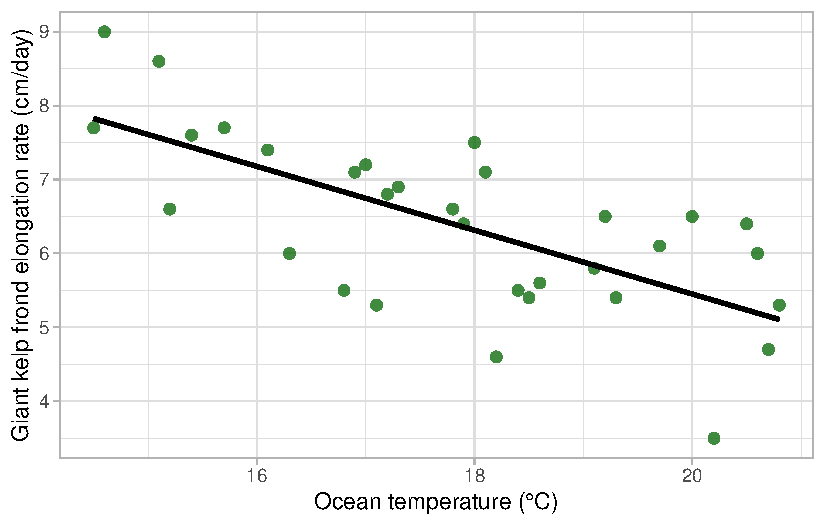
\includegraphics[keepaspectratio]{HW3_files/figure-pdf/unnamed-chunk-2-1.pdf}}

\subsection{c.~Check your assumptions and run your
test}\label{c.-check-your-assumptions-and-run-your-test}

\subsubsection{Check assumptions}\label{check-assumptions}

\begin{Shaded}
\begin{Highlighting}[]
\CommentTok{\#Create a linear regression model}
\NormalTok{kelp\_lm }\OtherTok{\textless{}{-}} \FunctionTok{lm}\NormalTok{(kelp\_elong }\SpecialCharTok{\textasciitilde{}}\NormalTok{ temp\_c,}
              \AttributeTok{data =}\NormalTok{ kelp)}

\CommentTok{\#Create a diagnostic plots to check model assumptions}
\FunctionTok{plot}\NormalTok{(kelp\_lm)}
\end{Highlighting}
\end{Shaded}

\pandocbounded{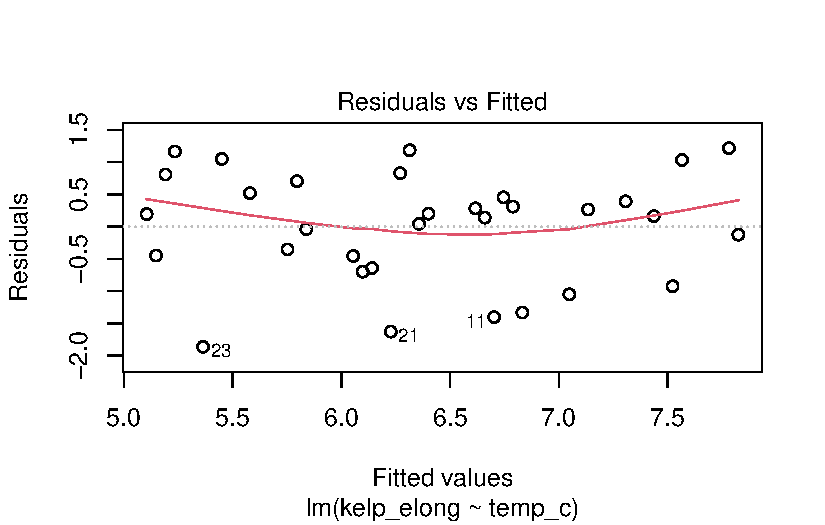
\includegraphics[keepaspectratio]{HW3_files/figure-pdf/unnamed-chunk-3-1.pdf}}

\pandocbounded{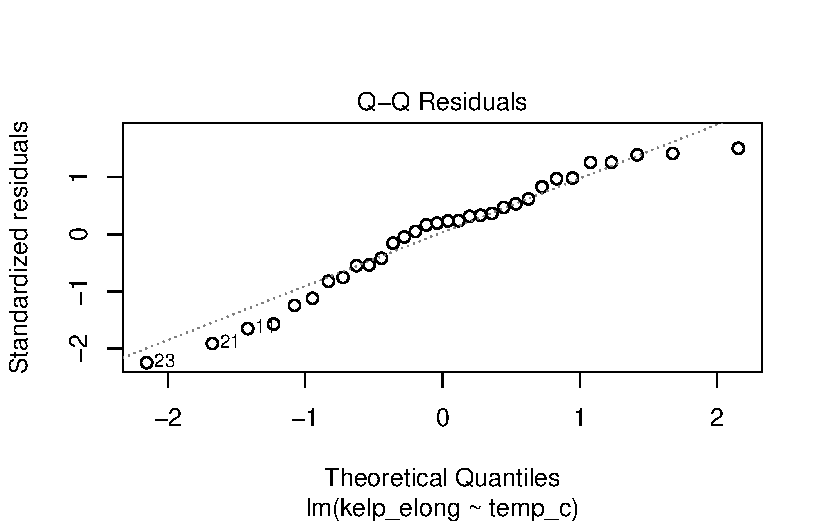
\includegraphics[keepaspectratio]{HW3_files/figure-pdf/unnamed-chunk-3-2.pdf}}

\pandocbounded{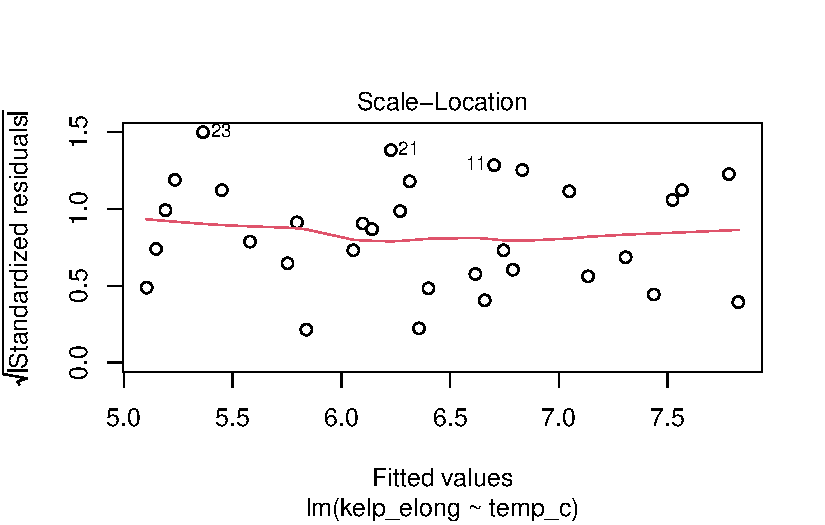
\includegraphics[keepaspectratio]{HW3_files/figure-pdf/unnamed-chunk-3-3.pdf}}

\pandocbounded{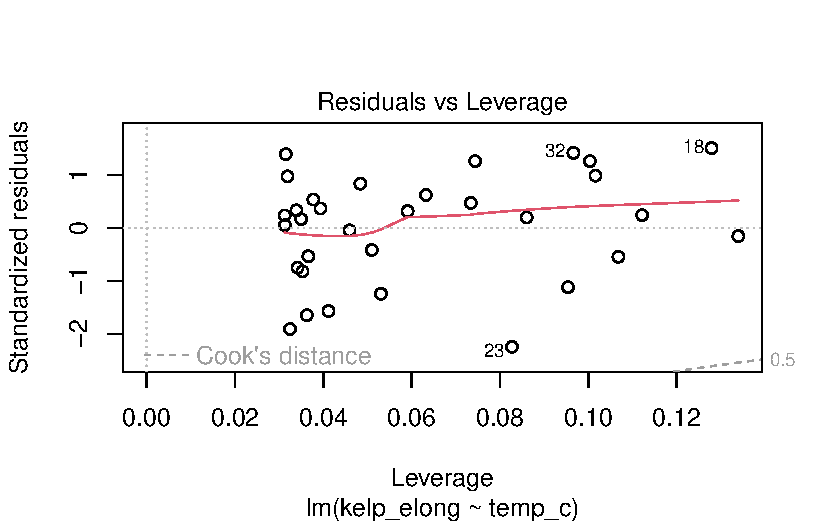
\includegraphics[keepaspectratio]{HW3_files/figure-pdf/unnamed-chunk-3-4.pdf}}

I checked the linearity assumption with the use of the scatterplot,
which displayed a generally negative relationship between ocean
temperature and giant kelp frond elongation rate. I then checked the
assumptions using the diagnostic plots from the linear model, including
the residuals vs.~fitted plot, Q-Q plot, scale-location plot, and
residuals vs.~leverage plot. The residuals vs.~fitted plot displayed a
slight curve in the smoothed trend line, although there was no extreme
plattern and the residuals were mostly spread around 0, so is reasonable
to continue with a simple linear regression.

\subsubsection{Run test}\label{run-test}

\begin{Shaded}
\begin{Highlighting}[]
\CommentTok{\#Summarize the linear regression model}
\FunctionTok{summary}\NormalTok{(kelp\_lm)}
\end{Highlighting}
\end{Shaded}

\begin{verbatim}

Call:
lm(formula = kelp_elong ~ temp_c, data = kelp)

Residuals:
    Min      1Q  Median      3Q     Max 
-1.8643 -0.5017  0.1790  0.5659  1.2177 

Coefficients:
            Estimate Std. Error t value Pr(>|t|)    
(Intercept) 14.08645    1.49219   9.440 1.72e-10 ***
temp_c      -0.43179    0.08321  -5.189 1.37e-05 ***
---
Signif. codes:  0 '***' 0.001 '**' 0.01 '*' 0.05 '.' 0.1 ' ' 1

Residual standard error: 0.8665 on 30 degrees of freedom
Multiple R-squared:  0.473, Adjusted R-squared:  0.4554 
F-statistic: 26.93 on 1 and 30 DF,  p-value: 1.366e-05
\end{verbatim}

\subsection{d.~Results communication}\label{d.-results-communication}

In order to evaluate the strength of the relationship between
temperature and giant kelp frond elongation rate, I used a simple linear
regression, as kelp frond elongation rate is a continuous response
variable and ocean temperature is a continuous predictor variable. The
results suggest that ocean temperature significantly predicted kelp
frond elongation rate (linear model: F(1, 30) = 26.93, p \textless{}
0.001, \(\alpha = 0.05\), adjusted R² = 0.455). Therefore, for each 1°C
increase in ocean temperature, one would expect a decrease in giant kelp
frond elongation rate by 0.432 ± 0.083 (SE) cm/day.

\subsection{e. Test implications}\label{e.-test-implications}

I would communicate to the team that higher ocean temperatures were
generally associated with lower giant kelp frond elongation rates,
according to this data set. As kelp elongation rate was shown to
decrease by 0.432 cm/day for each 1°C increase in ocean temperature,
areas with warmer ocean conditions may be prudent to monitor when
looking at its relationship to~kelp growth and overall kelp forest
health. Despite this, as the study is based on one observational data
set, it is important to communicate that this result shows an
association rather than proving a causation.

\subsection{f.~Double check your own
work}\label{f.-double-check-your-own-work}

\begin{Shaded}
\begin{Highlighting}[]
\CommentTok{\#Run a Pearson correlation test to test the strength of the relationship}
\FunctionTok{cor.test}\NormalTok{(}\AttributeTok{x =}\NormalTok{ kelp}\SpecialCharTok{$}\NormalTok{temp\_c,}
         \AttributeTok{y =}\NormalTok{ kelp}\SpecialCharTok{$}\NormalTok{kelp\_elong,}
         \AttributeTok{method =} \StringTok{"pearson"}\NormalTok{)}
\end{Highlighting}
\end{Shaded}

\begin{verbatim}

    Pearson's product-moment correlation

data:  kelp$temp_c and kelp$kelp_elong
t = -5.189, df = 30, p-value = 1.366e-05
alternative hypothesis: true correlation is not equal to 0
95 percent confidence interval:
 -0.8359665 -0.4460157
sample estimates:
       cor 
-0.6877489 
\end{verbatim}

Both the Pearson correlation test and simple linear regression tests
reject the null hypothesis, as both tests suggest a statistically
significant negative relationship between ocean temperature and giant
kelp frond elongation rate. The Pearson correlation test displays a
moderately strong negative relationship between ocean temperature and
giant kelp frond elongation rate (Pearson's r = -0.688, t(30) = -5.19, p
\textless{} 0.001, \(\alpha = 0.05\)). This conclusion is in alignment
with the results of the simple linear regression test, as they both
suggest that kelp frond elongation rate decreased as ocean temperature
increased.

\section{Problem 2. Personal data}\label{problem-2.-personal-data}

\subsection{a. Updating your
visualizations}\label{a.-updating-your-visualizations}

\subsubsection{Productivity by day of the
week}\label{productivity-by-day-of-the-week}

\begin{Shaded}
\begin{Highlighting}[]
\CommentTok{\#Define a productivity column as a percentage}
\NormalTok{personal\_data }\OtherTok{\textless{}{-}}\NormalTok{ personal\_data }\SpecialCharTok{|\textgreater{}}
  \FunctionTok{mutate}\NormalTok{(}\AttributeTok{productivity =}\NormalTok{ tasks\_completed }\SpecialCharTok{/}\NormalTok{ tasks\_planned }\SpecialCharTok{*} \DecValTok{100}\NormalTok{)}

\CommentTok{\#Create a boxplot to display productivity versus day of the week}
\FunctionTok{ggplot}\NormalTok{(}\AttributeTok{data =}\NormalTok{ personal\_data,}
       \AttributeTok{mapping =} \FunctionTok{aes}\NormalTok{(}\AttributeTok{x =} \FunctionTok{factor}\NormalTok{(day\_of\_week,}
                                \AttributeTok{levels =} \FunctionTok{c}\NormalTok{(}\StringTok{"Monday"}\NormalTok{,}
                                           \StringTok{"Tuesday"}\NormalTok{,}
                                           \StringTok{"Wednesday"}\NormalTok{,}
                                           \StringTok{"Thursday"}\NormalTok{,}
                                           \StringTok{"Friday"}\NormalTok{,}
                                           \StringTok{"Saturday"}\NormalTok{,}
                                           \StringTok{"Sunday"}\NormalTok{)),}
                     \AttributeTok{y =}\NormalTok{ productivity)) }\SpecialCharTok{+}

\CommentTok{\#Set y{-}axis limits to show full range}
\FunctionTok{scale\_y\_continuous}\NormalTok{(}\AttributeTok{limits =} \FunctionTok{c}\NormalTok{(}\DecValTok{0}\NormalTok{, }\DecValTok{100}\NormalTok{)) }\SpecialCharTok{+}

\CommentTok{\#Add boxplots to summarize productivity depending on each day}
\FunctionTok{geom\_boxplot}\NormalTok{(}\AttributeTok{fill =} \StringTok{"steelblue"}\NormalTok{) }\SpecialCharTok{+}

\CommentTok{\#Relabel both axes and add most recent observation date}
\FunctionTok{labs}\NormalTok{(}\AttributeTok{x =} \StringTok{"Day of the week"}\NormalTok{,}
     \AttributeTok{y =} \StringTok{"Productivity level (\%)"}\NormalTok{,}
     \AttributeTok{title =} \StringTok{"Productivity by Day of the Week"}\NormalTok{,}
     \AttributeTok{subtitle =} \StringTok{"Most recent observation: 2026{-}05{-}26"}\NormalTok{) }\SpecialCharTok{+}

\CommentTok{\#Change theme}
\FunctionTok{theme\_light}\NormalTok{() }\SpecialCharTok{+}
  
\CommentTok{\#Center title and subtitle and make x{-}axis smaller}
\FunctionTok{theme}\NormalTok{(}\AttributeTok{plot.title =} \FunctionTok{element\_text}\NormalTok{(}\AttributeTok{hjust =} \FloatTok{0.5}\NormalTok{),}
      \AttributeTok{plot.subtitle =} \FunctionTok{element\_text}\NormalTok{(}\AttributeTok{hjust =} \FloatTok{0.5}\NormalTok{),}
      \AttributeTok{axis.text.x =} \FunctionTok{element\_text}\NormalTok{(}\AttributeTok{size =} \DecValTok{7}\NormalTok{))}
\end{Highlighting}
\end{Shaded}

\pandocbounded{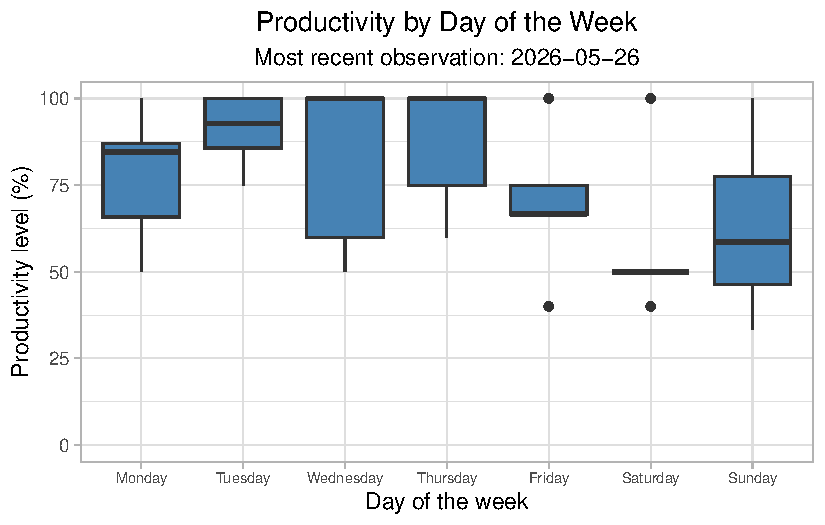
\includegraphics[keepaspectratio]{HW3_files/figure-pdf/unnamed-chunk-6-1.pdf}}

\subsubsection{Productivity versus
sleep}\label{productivity-versus-sleep}

\begin{Shaded}
\begin{Highlighting}[]
\CommentTok{\#Create a scatterplot to display relationship between sleep and productivity (tasks completed/tasks planned)}
\FunctionTok{ggplot}\NormalTok{(}\AttributeTok{data =}\NormalTok{ personal\_data,}
       \AttributeTok{mapping =} \FunctionTok{aes}\NormalTok{(}\AttributeTok{x =}\NormalTok{ sleep\_minutes,}
                     \AttributeTok{y =}\NormalTok{ productivity)) }\SpecialCharTok{+}

\CommentTok{\#Add one point for each daily observation from data set}
\FunctionTok{geom\_point}\NormalTok{(}\AttributeTok{color =} \StringTok{"darkgreen"}\NormalTok{,}
           \AttributeTok{size =} \DecValTok{2}\NormalTok{,}
           \AttributeTok{alpha =} \FloatTok{0.75}\NormalTok{) }\SpecialCharTok{+}

\CommentTok{\#Add a linear trend line to display relationship}
\FunctionTok{geom\_smooth}\NormalTok{(}\AttributeTok{method =} \StringTok{"lm"}\NormalTok{,}
            \AttributeTok{se =} \ConstantTok{FALSE}\NormalTok{,}
            \AttributeTok{color =} \StringTok{"black"}\NormalTok{) }\SpecialCharTok{+}

\CommentTok{\#Relabel both axes and insert most recent observation date}
\FunctionTok{labs}\NormalTok{(}\AttributeTok{x =} \StringTok{"Sleep (minutes)"}\NormalTok{,}
     \AttributeTok{y =} \StringTok{"Productivity level (\%)"}\NormalTok{,}
     \AttributeTok{title =} \StringTok{"Productivity versus Sleep"}\NormalTok{,}
     \AttributeTok{subtitle =} \StringTok{"Most recent observation: 2026{-}05{-}26"}\NormalTok{) }\SpecialCharTok{+}

\CommentTok{\#Change theme}
\FunctionTok{theme\_light}\NormalTok{() }\SpecialCharTok{+}

\CommentTok{\#Center the title and subtitle}
\FunctionTok{theme}\NormalTok{(}\AttributeTok{plot.title =} \FunctionTok{element\_text}\NormalTok{(}\AttributeTok{hjust =} \FloatTok{0.5}\NormalTok{),}
      \AttributeTok{plot.subtitle =} \FunctionTok{element\_text}\NormalTok{(}\AttributeTok{hjust =} \FloatTok{0.5}\NormalTok{))}
\end{Highlighting}
\end{Shaded}

\pandocbounded{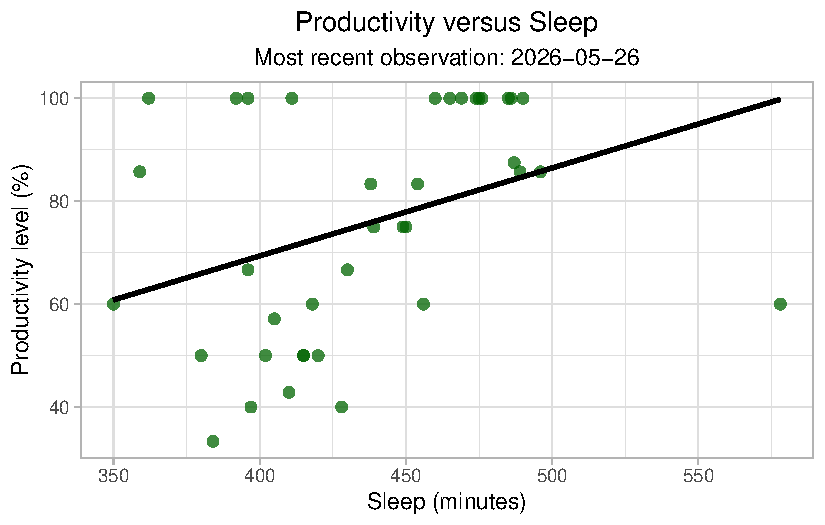
\includegraphics[keepaspectratio]{HW3_files/figure-pdf/unnamed-chunk-7-1.pdf}}

\subsection{b. Captions}\label{b.-captions}

\textbf{Figure 1. Productivity level varied by day of the week across
the personal data collection period.} Blue boxplots display the median
and interquartile range of productivity level, measured as a percentage
of tasks completed out of tasks planned at the beginning of the day, for
each day of the week. Data were derived from personal observations
collected from 2026-04-19 to 2026-05-26. Data accessed 2026-05-28.

\textbf{Figure 2. Productivity level generally increased as sleep
increased throughout the personal data collection period.} Transparent
dark green points represent daily observations of sleep, in minutes, and
productivity level, measured as a percentage of tasks completed out of
tasks planned at the beginning of the day. The black line shows the
linear trend between sleep and productivity. Data were derived from
personal observations collected from 2026-04-19 to 2026-05-26. Data
accessed 2026-05-28.

\section{Problem 3. Affective
visualization}\label{problem-3.-affective-visualization}

\subsection{a. Describe in words what an affective visualization could
look like for your personal
data}\label{a.-describe-in-words-what-an-affective-visualization-could-look-like-for-your-personal-data}

For my affective visualization, I am thinking of creating a
3-dimensional model of a skyline, where exposure to light represents
productivity level and the height of each building represents a range of
minutes of sleep. I would orientate the buildings in a parallel line so
the tallest building (representing most sleep) would be at the front,
and closest to the light (representing the sun), meaning it would
therefore be the most lit up. The subsequent buildings would then be
partially covered by the building in front of them and receive less
light, so the smallest building (representing the least sleep) would be
the darkest and represent lower productivity. The angle of the trend
line should follow the angle of descending buildings on the skyline as
to properly explore the relationship between sleep and productivity
level.

\subsection{b. Create a sketch (on paper) of your
idea.}\label{b.-create-a-sketch-on-paper-of-your-idea.}

\begin{figure}[H]

{\centering \pandocbounded{
\includegraphics[keepaspectratio]{./Users/owenwright/Downloads/IMG_1282.heic}}

}

\caption{Sketch of affective visualization}

\end{figure}%




\end{document}
